\PassOptionsToPackage{english,ngerman}{babel}

\documentclass[a4paper,11pt]{article}

\usepackage{../style/thga-db}

% ============================================================
% Document metadata
% ============================================================

\renewcommand{\thgaKurs}{User Manual -- Filament Manager}
\renewcommand{\thgaDozent}{Stephan Bökelmann}
\renewcommand{\thgaEmail}{sboekelmann@ep1.rub.de}
\renewcommand{\thgaDatum}{\today}

% ------------------------------------------------------------
% Custom header and footer for the User Manual
% ------------------------------------------------------------

\fancyhead[L]{%
  \small\textcolor{THGABlau}{%
    \textbf{User Manual -- Filament Manager}%
  }%
}

\fancyhead[R]{%
  \small\textcolor{THGAGrau}{%
    Daniel Brendebach \ · \ \thgaDatum%
  }%
}

\fancyfoot[L]{}
\fancyfoot[C]{%
  \small\textcolor{THGAGrau}{THGA Bochum}%
}
\fancyfoot[R]{%
  \small\textcolor{THGAGrau}{\thepage}%
}

\hypersetup{
  pdftitle={Filament Manager -- User Manual},
  pdfauthor={Daniel Brendebach},
  pdfsubject={User documentation for the Filament Manager},
}

\begin{document}

\selectlanguage{english}

% ============================================================
% Title
% ============================================================

\thispagestyle{empty}

\thgaTitel
  {Filament Manager}
  {User Manual}

\vspace{0.8cm}

\begin{tabularx}{\linewidth}{@{}lX@{}}
\textbf{Author:}      & Daniel Brendebach \\
\textbf{Document:}    & User Manual \\
\textbf{Version:}     & 1.0 \\
\textbf{Application:} & Filament Manager \\
\textbf{Module:}      & Datenbanken \\
\textbf{Date:}        & \today \\
\end{tabularx}

\vfill

\begin{infobox}
This manual explains how to install, start and operate the Filament Manager
desktop application. It is intended for end users who want to manage filament
rolls, filament types, print models, stock and print jobs without interacting
directly with the database or REST API.
\end{infobox}

\newpage

% ============================================================
% Table of contents
% ============================================================

\tableofcontents

\newpage

% ============================================================
\section{Introduction}
% ============================================================

The Filament Manager is a desktop application for managing filament used for
3D printing.

The application allows users to:

\begin{itemize}
  \item manage physical filament rolls,
  \item manage filament types,
  \item manage print models,
  \item view the current filament stock,
  \item start print jobs,
  \item view the print history.
\end{itemize}

The desktop application communicates with a separate backend server. The user
does not need direct access to the PostgreSQL database.

All normal operations are performed through the graphical user interface.

% ============================================================
\section{System requirements}
% ============================================================

The Filament Manager frontend is intended for Linux systems based on Debian
or compatible distributions.

A normal installation requires:

\begin{itemize}
  \item a Linux desktop system,
  \item network access to the Filament Manager backend,
  \item the Filament Manager Debian package,
  \item the backend address,
  \item the API key for write operations.
\end{itemize}

The backend must be running before the desktop application can load or modify
data.

% ============================================================
\section{Installation}
% ============================================================

The desktop frontend is distributed as a Debian package.

Assume the package file is called:

\begin{lstlisting}
filament-manager-frontend_0.1.0_all.deb
\end{lstlisting}

Open a terminal in the directory containing the package and run:

\begin{lstlisting}
sudo apt install ./filament-manager-frontend_0.1.0_all.deb
\end{lstlisting}

The system may ask for the user's administrator password.

After successful installation, the application command is available globally:

\begin{lstlisting}
filament-manager-frontend
\end{lstlisting}

\begin{infobox}
The desktop application and backend are separate components. Installing the
frontend does not automatically install or start the backend server.
\end{infobox}

% ============================================================
\section{Starting the application}
% ============================================================

Start the application from a terminal with:

\begin{lstlisting}
filament-manager-frontend
\end{lstlisting}

The application first opens the connection dialog shown in
Figure~\ref{fig:connection-dialog}.

\begin{figure}[htbp]
  \centering
  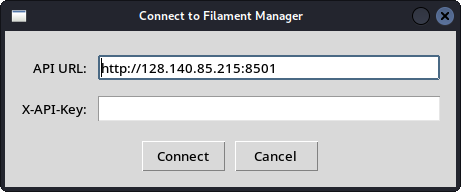
\includegraphics[
    width=0.62\textwidth,
    height=0.45\textheight,
    keepaspectratio
  ]{images/connection-dialog.png}
  \caption{Connection dialog shown when the application starts}
  \label{fig:connection-dialog}
\end{figure}

% ============================================================
\section{Connecting to the backend}
% ============================================================

The connection dialog requires the backend address and API key.

\subsection{Backend URL}

The backend URL identifies the computer on which the Filament Manager backend
is running.

For a backend running on the same computer:

\begin{lstlisting}
http://localhost:8501
\end{lstlisting}

For a backend on another computer:

\begin{lstlisting}
http://<server-address>:8501
\end{lstlisting}

Replace \texttt{<server-address>} with the hostname or IP address supplied by
the administrator.

\subsection{API key}

The API key is required for operations that modify data, such as:

\begin{itemize}
  \item adding a filament roll,
  \item deleting a filament roll,
  \item adding or deleting filament types,
  \item adding or deleting print models,
  \item starting a print.
\end{itemize}

Enter the API key supplied by the backend administrator.

\begin{warnbox}
Do not share the API key with unauthorised users. The key permits changes to
the Filament Manager data.
\end{warnbox}

After entering the connection information, use the connection button in the
dialog.

If the connection succeeds, the main application window opens.

% ============================================================
\section{Main application window}
% ============================================================

The main window is organised using several tabs.

The available tabs are:

\begin{itemize}
  \item \textbf{Filament Rolls},
  \item \textbf{Filament Types},
  \item \textbf{Print Models},
  \item \textbf{Stock},
  \item \textbf{Print History}.
\end{itemize}

Each tab represents one functional area of the application.

% ============================================================
\section{Filament Rolls}
% ============================================================

The \textbf{Filament Rolls} tab manages individual physical filament spools.

Figure~\ref{fig:filament-rolls} shows the filament roll overview.

\begin{figure}[htbp]
  \centering
  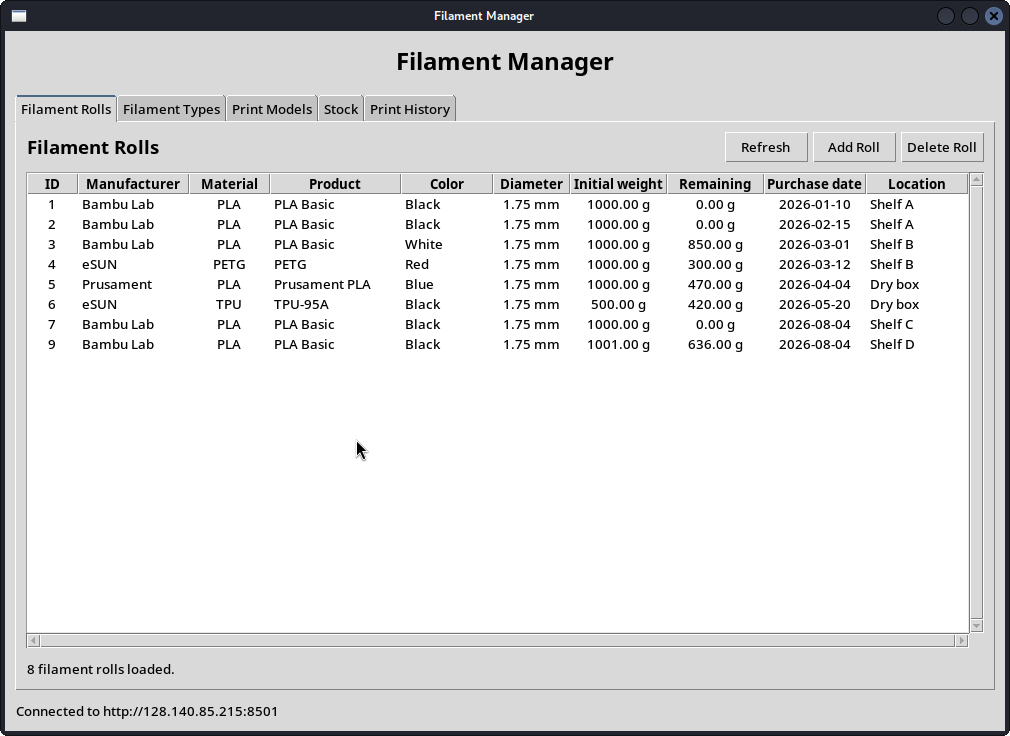
\includegraphics[
    width=\textwidth,
    height=0.56\textheight,
    keepaspectratio
  ]{images/filament-rolls.png}
  \caption{Filament Rolls overview}
  \label{fig:filament-rolls}
\end{figure}

The table displays information such as:

\begin{itemize}
  \item roll ID,
  \item manufacturer,
  \item material,
  \item product name,
  \item colour,
  \item diameter,
  \item initial weight,
  \item remaining weight,
  \item purchase date,
  \item storage location.
\end{itemize}

\subsection{Refresh filament rolls}

Use the \textbf{Refresh} button to reload the current list from the backend.

This is useful if data was changed from another client.

\subsection{Adding a filament roll}

Select \textbf{Add Roll}.

The dialog shown in Figure~\ref{fig:add-roll} opens.

\begin{figure}[htbp]
  \centering
  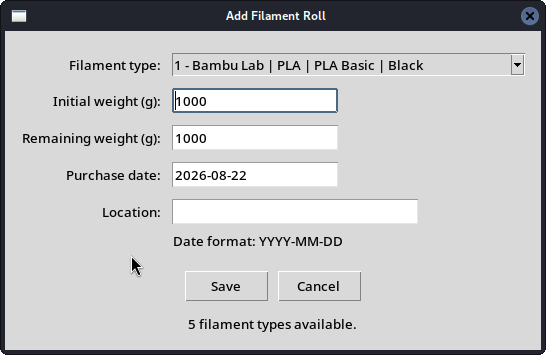
\includegraphics[
    width=0.66\textwidth,
    height=0.55\textheight,
    keepaspectratio
  ]{images/add-roll.png}
  \caption{Dialog for adding a new filament roll}
  \label{fig:add-roll}
\end{figure}

Enter the required information.

The filament type must already exist before a physical roll can be created.

Typical fields include:

\begin{itemize}
  \item filament type,
  \item initial weight,
  \item remaining weight,
  \item purchase date,
  \item storage location.
\end{itemize}

For a newly purchased roll, the initial and remaining weight will normally be
identical.

Example:

\begin{lstlisting}
Initial weight:   1000 g
Remaining weight: 1000 g
Location:         Shelf A
\end{lstlisting}

Confirm the dialog to save the roll.

After successful creation, the roll appears in the overview.

\subsection{Deleting a filament roll}

Select the desired row in the table and press \textbf{Delete Roll}.

The application asks for confirmation before sending the delete request.

A roll can only be deleted if it is not required by existing print history.

If the roll has already been used by a recorded print job, the backend
protects the historical data and rejects the deletion.

In this case, the application displays an error message and the roll remains
in the database.

% ============================================================
\section{Filament Types}
% ============================================================

A filament type describes the product characteristics shared by one or more
physical rolls.

This includes:

\begin{itemize}
  \item manufacturer,
  \item material,
  \item product name,
  \item colour,
  \item filament diameter.
\end{itemize}

Figure~\ref{fig:filament-types} shows the filament type overview.

\begin{figure}[htbp]
  \centering
  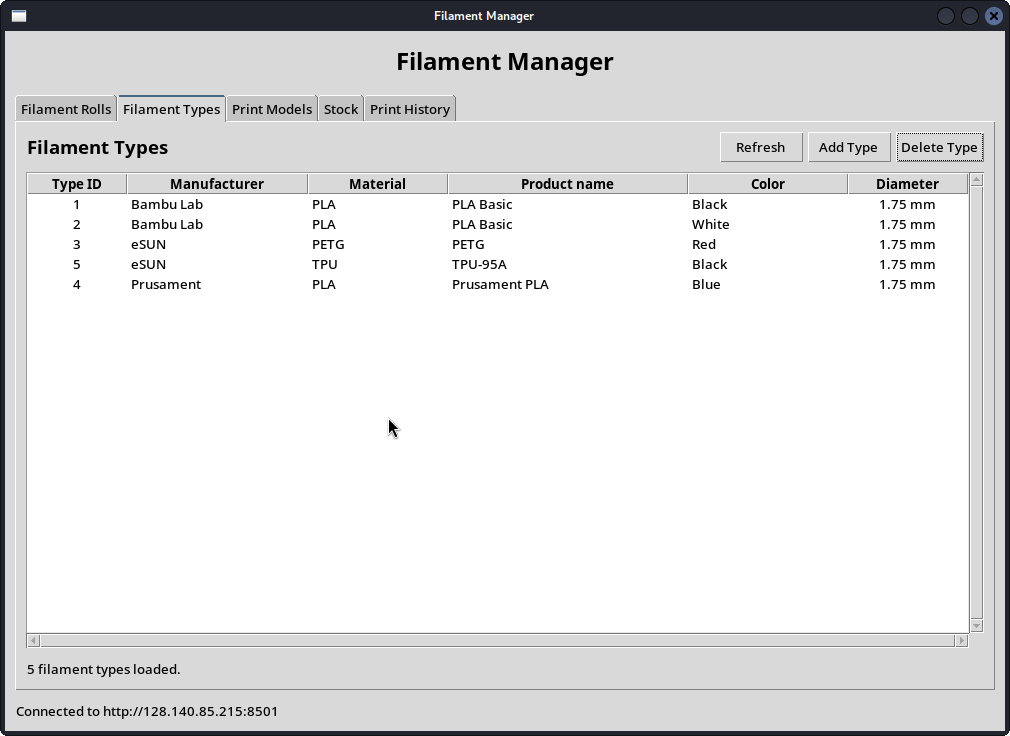
\includegraphics[
    width=\textwidth,
    height=0.56\textheight,
    keepaspectratio
  ]{images/filament-types.png}
  \caption{Filament Types overview}
  \label{fig:filament-types}
\end{figure}

\subsection{Adding a filament type}

Press \textbf{Add Type}.

The dialog shown in Figure~\ref{fig:add-filament-type} opens.

\begin{figure}[htbp]
  \centering
  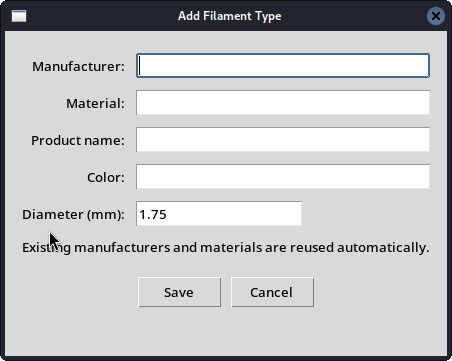
\includegraphics[
    width=0.64\textwidth,
    height=0.52\textheight,
    keepaspectratio
  ]{images/add-filament-type.png}
  \caption{Dialog for creating a filament type}
  \label{fig:add-filament-type}
\end{figure}

Enter:

\begin{itemize}
  \item manufacturer,
  \item material,
  \item product name,
  \item colour,
  \item diameter.
\end{itemize}

A common filament diameter is:

\begin{lstlisting}
1.75 mm
\end{lstlisting}

Existing manufacturer and material entries are reused automatically by the
backend where applicable.

After the new type has been created, it can be selected when adding a
filament roll.

\subsection{Deleting a filament type}

Select a filament type and press \textbf{Delete Type}.

A confirmation dialog is shown.

A filament type cannot be deleted while physical filament rolls still
reference it.

If such rolls exist, the backend rejects the operation and the application
shows the corresponding error message.

To remove the type, the dependent rolls would first have to be removed,
provided they themselves are not protected by existing print history.

% ============================================================
\section{Print Models}
% ============================================================

The \textbf{Print Models} tab stores reusable information about objects that
can be printed.

Figure~\ref{fig:print-models} shows the print model overview.

\begin{figure}[htbp]
  \centering
  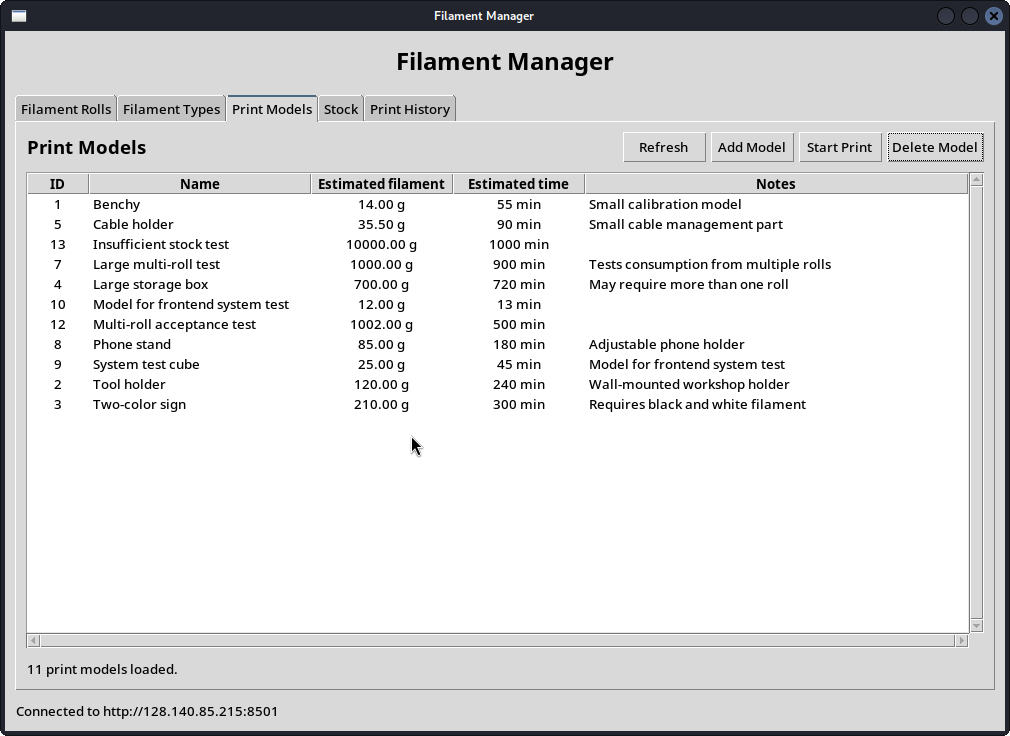
\includegraphics[
    width=\textwidth,
    height=0.56\textheight,
    keepaspectratio
  ]{images/print-models.png}
  \caption{Print Models overview}
  \label{fig:print-models}
\end{figure}

A print model can contain:

\begin{itemize}
  \item model name,
  \item estimated filament consumption,
  \item estimated print time,
  \item notes.
\end{itemize}

The estimated filament amount is later used automatically when a print job is
started.

\subsection{Adding a print model}

Press \textbf{Add Model}.

The dialog shown in Figure~\ref{fig:add-model} opens.

\begin{figure}[htbp]
  \centering
  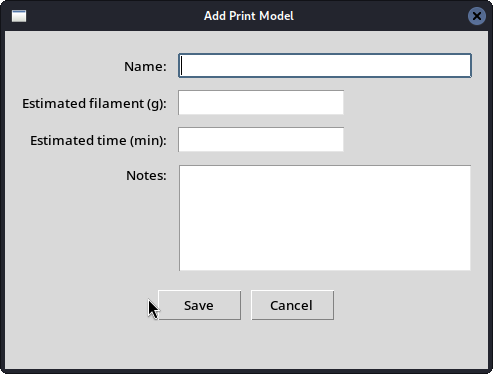
\includegraphics[
    width=0.66\textwidth,
    height=0.52\textheight,
    keepaspectratio
  ]{images/add-model.png}
  \caption{Dialog for adding a print model}
  \label{fig:add-model}
\end{figure}

Enter the model information.

Example:

\begin{lstlisting}
Name:               Cable holder
Estimated filament: 35.5 g
Estimated time:     90 min
Notes:              Small cable management part
\end{lstlisting}

The filament estimate must be greater than zero.

After saving, the model appears in the model table.

\subsection{Deleting a print model}

Select a model and press \textbf{Delete Model}.

Confirm the requested deletion.

A model that is already referenced by print history cannot be deleted,
because doing so would invalidate historical print records.

If the model is still in use, the backend rejects the request.

% ============================================================
\section{Starting a Print}
% ============================================================

A print job can be started from the \textbf{Print Models} tab.

Select the required model and press \textbf{Start Print}.

A model can also be selected before opening the dialog, depending on the
current application state.

The print dialog is shown in Figure~\ref{fig:start-print}.

\begin{figure}[htbp]
  \centering
  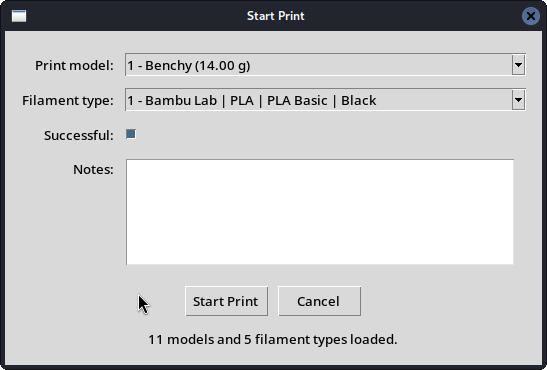
\includegraphics[
    width=0.68\textwidth,
    height=0.58\textheight,
    keepaspectratio
  ]{images/start-print.png}
  \caption{Dialog for starting a print job}
  \label{fig:start-print}
\end{figure}

\subsection{Selecting the model}

The print model determines the estimated filament weight required for the
job.

For example, if the selected model has:

\begin{lstlisting}
Estimated filament: 120 g
\end{lstlisting}

the backend attempts to allocate \texttt{120 g} of the selected filament
type.

\subsection{Selecting the filament type}

Select the filament type that should be used for the print.

The backend considers only physical rolls belonging to this exact filament
type.

\subsection{Successful print setting}

The dialog allows the print to be recorded as successful or unsuccessful,
depending on the available option in the application.

Notes can also be added to the print job where required.

\subsection{Automatic roll selection}

The user does not manually select the physical roll that is consumed.

The backend automatically chooses suitable rolls.

If one physical roll contains enough filament, the backend uses the smallest
roll that can complete the print.

Example:

\begin{lstlisting}
Available rolls:
180 g
620 g
950 g

Required:
500 g

Selected:
620 g roll
\end{lstlisting}

This avoids consuming filament from a larger roll unnecessarily.

\subsection{Prints requiring multiple rolls}

If no single roll contains enough filament but several rolls together contain
a sufficient amount, the backend can allocate multiple rolls.

For example:

\begin{lstlisting}
Required: 1000 g

Allocation:
Roll 1: 166 g
Roll 2: 620 g
Roll 7: 214 g
\end{lstlisting}

The user does not need to calculate this distribution manually.

When the print job is created, the allocated quantities are deducted from the
corresponding filament rolls.

\subsection{Insufficient filament}

If the total available filament of the selected type is smaller than the
required model weight, the print cannot be created.

The application displays an error message.

No filament is deducted and no incomplete print record is created.

\begin{infobox}
The remaining filament values are only changed after the backend has verified
that enough filament is available for the complete print.
\end{infobox}

% ============================================================
\section{Stock Overview}
% ============================================================

The \textbf{Stock} tab displays aggregated filament inventory.

Figure~\ref{fig:stock} shows the stock overview.

\begin{figure}[htbp]
  \centering
  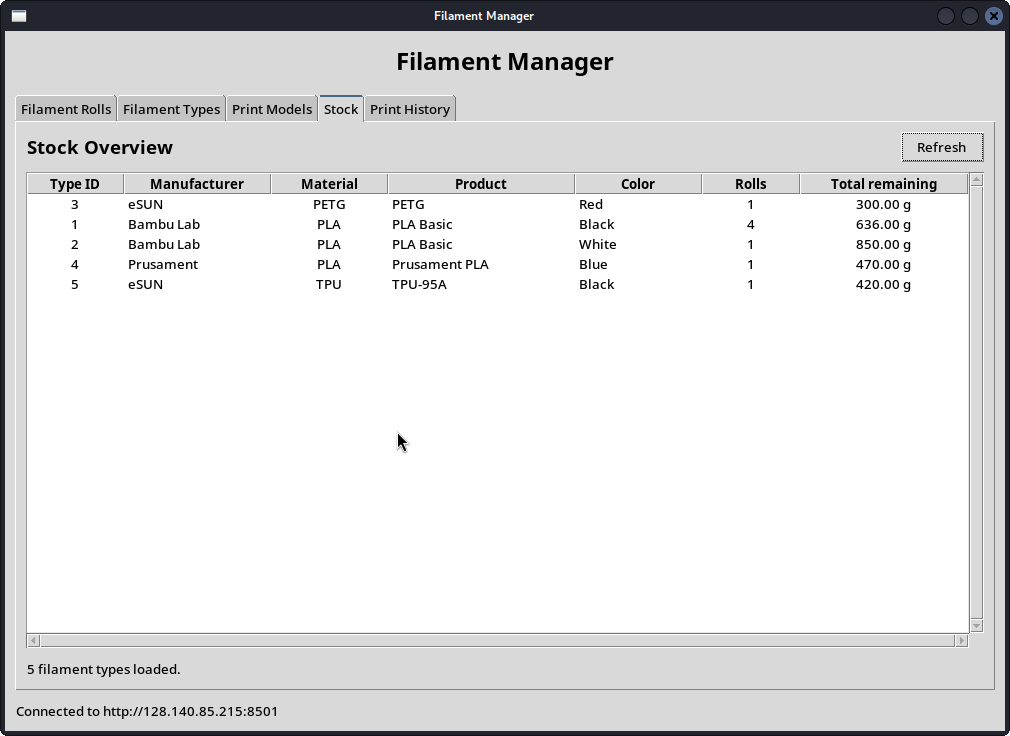
\includegraphics[
    width=\textwidth,
    height=0.56\textheight,
    keepaspectratio
  ]{images/stock.png}
  \caption{Aggregated filament stock overview}
  \label{fig:stock}
\end{figure}

Unlike the Filament Rolls tab, the Stock tab does not show every physical roll
individually.

Instead, rolls of the same filament type are combined.

Typical displayed information includes:

\begin{itemize}
  \item manufacturer,
  \item material,
  \item product name,
  \item colour,
  \item number of rolls,
  \item total remaining filament weight.
\end{itemize}

Example:

\begin{lstlisting}
Bambu Lab
PLA
PLA Basic
Black
2 rolls
800 g total remaining
\end{lstlisting}

Use \textbf{Refresh} to reload the current inventory from the backend.

After a new print job has been created, the stock values are updated to
reflect the consumed filament.

% ============================================================
\section{Print History}
% ============================================================

The \textbf{Print History} tab shows recorded print jobs.

Figure~\ref{fig:print-history} shows the history view.

\begin{figure}[htbp]
  \centering
  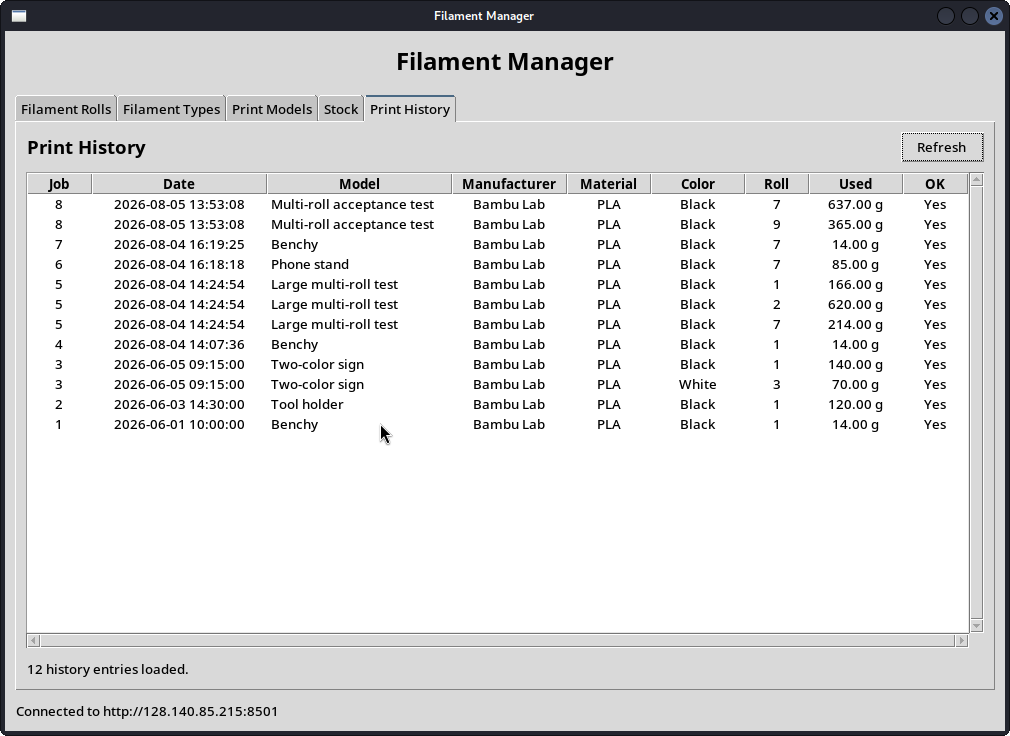
\includegraphics[
    width=\textwidth,
    height=0.58\textheight,
    keepaspectratio
  ]{images/print-history.png}
  \caption{Print History overview}
  \label{fig:print-history}
\end{figure}

The history contains information such as:

\begin{itemize}
  \item print job ID,
  \item print date,
  \item model,
  \item success status,
  \item notes,
  \item filament roll,
  \item filament type information,
  \item amount of filament consumed.
\end{itemize}

A print job that used multiple physical rolls can appear in more than one row.

For example, one job may be displayed as:

\begin{lstlisting}
Job 5 | Roll 1 | 166 g
Job 5 | Roll 2 | 620 g
Job 5 | Roll 7 | 214 g
\end{lstlisting}

These rows represent one print job that consumed filament from three rolls.

Use \textbf{Refresh} to reload the current print history.

% ============================================================
\section{Data relationships and deletion behaviour}
% ============================================================

Some records cannot be deleted because they are referenced by other data.

This behaviour is intentional and protects the consistency of the print
history.

\subsection{Filament types}

A filament type cannot normally be deleted while filament rolls reference it.

\subsection{Filament rolls}

A filament roll cannot normally be deleted once it is referenced by an
existing print job.

\subsection{Print models}

A print model cannot normally be deleted once it is referenced by an
existing print job.

\begin{infobox}
If a delete request is rejected, this does not indicate a broken application.
The backend is preserving related data required for a consistent print
history.
\end{infobox}

% ============================================================
\section{Typical workflow}
% ============================================================

A typical workflow for a new installation is:

\begin{enumerate}
  \item Start the application.
  \item Connect to the backend.
  \item Open \textbf{Filament Types}.
  \item Create the required filament types.
  \item Open \textbf{Filament Rolls}.
  \item Add the physical rolls currently available.
  \item Open \textbf{Print Models}.
  \item Create the required print models.
  \item Select a model and start a print.
  \item Select the required filament type.
  \item Confirm the print job.
  \item Check the updated stock.
  \item Open the print history to verify the recorded job.
\end{enumerate}

This workflow ensures that all required master data exists before a print is
started.

% ============================================================
\section{Error messages and troubleshooting}
% ============================================================

\subsection{The application cannot connect to the backend}

Possible causes include:

\begin{itemize}
  \item incorrect backend address,
  \item backend server is offline,
  \item backend containers are not running,
  \item port \texttt{8501} is blocked,
  \item no network connection exists between frontend and backend.
\end{itemize}

Check the configured backend URL.

A typical remote URL has the form:

\begin{lstlisting}
http://server-address:8501
\end{lstlisting}

Contact the backend administrator if the server is not reachable.

\subsection{Invalid or missing API key}

If a write operation is rejected because of the API key, verify the key
entered in the connection dialog.

The backend and frontend must use the same API key.

Read-only views may still work even if the write key is incorrect.

\subsection{Invalid input}

Some fields are validated before they are accepted.

Examples of invalid input include:

\begin{itemize}
  \item negative filament weight,
  \item zero filament requirement,
  \item invalid numeric values,
  \item missing required values.
\end{itemize}

Correct the value and repeat the operation.

\subsection{Not enough filament available}

If a print requires more filament than is currently available for the
selected type, the backend rejects the print.

Add another physical roll of the same filament type or select another
filament type with sufficient stock.

\subsection{A record cannot be deleted}

The requested object may already be referenced by another record.

Examples:

\begin{itemize}
  \item a filament type is referenced by a filament roll,
  \item a filament roll is referenced by print history,
  \item a print model is referenced by print history.
\end{itemize}

The protected record should normally remain in the system to preserve
historical consistency.

% ============================================================
\section{Closing the application}
% ============================================================

Close the main application window using the normal window close button.

The application does not require a separate logout procedure.

Connection information such as the API key is not intended to be permanently
stored by the application session after it is closed.

% ============================================================
\section{Updating the application}
% ============================================================

When a newer Debian package is provided, install it using the same package
manager command:

\begin{lstlisting}
sudo apt install ./filament-manager-frontend_<version>_all.deb
\end{lstlisting}

Replace \texttt{<version>} with the supplied package version.

The package manager performs the installation of the new application version.

The backend data is stored separately and is not part of the frontend Debian
package.

% ============================================================
\section{Uninstallation}
% ============================================================

Remove the desktop application with:

\begin{lstlisting}
sudo apt remove filament-manager-frontend
\end{lstlisting}

This removes the frontend application from the local Linux system.

It does not delete data stored on the backend PostgreSQL server.

\begin{warnbox}
Uninstalling the desktop frontend does not remove filament rolls, models,
filament types or print history from the backend database.
\end{warnbox}

% ============================================================
\section{Quick reference}
% ============================================================

\begin{tabularx}{\linewidth}{@{}p{4.2cm}X@{}}
\toprule
\textbf{Task} & \textbf{Location} \\
\midrule

View individual filament rolls
  & Filament Rolls tab \\

Add a physical roll
  & Filament Rolls $\rightarrow$ Add Roll \\

Delete an unused roll
  & Filament Rolls $\rightarrow$ Delete Roll \\

View filament types
  & Filament Types tab \\

Create a filament type
  & Filament Types $\rightarrow$ Add Type \\

Delete an unused type
  & Filament Types $\rightarrow$ Delete Type \\

View print models
  & Print Models tab \\

Create a model
  & Print Models $\rightarrow$ Add Model \\

Delete an unused model
  & Print Models $\rightarrow$ Delete Model \\

Start a print
  & Print Models $\rightarrow$ Start Print \\

View aggregated inventory
  & Stock tab \\

View completed print records
  & Print History tab \\

Reload displayed information
  & Refresh button on the corresponding tab \\

\bottomrule
\end{tabularx}

% ============================================================
\section{Summary}
% ============================================================

The Filament Manager provides a graphical interface for managing the most
important data required for filament-based 3D printing.

The user works exclusively through the desktop interface. The backend handles
database access, validation, filament allocation and consistency checks.

The normal operating sequence is:

\begin{center}
\textbf{Connect}
$\rightarrow$
\textbf{Manage filament}
$\rightarrow$
\textbf{Manage models}
$\rightarrow$
\textbf{Start print}
$\rightarrow$
\textbf{Review stock and history}
\end{center}

The application automatically selects suitable physical filament rolls when
a print job is created and prevents operations that would invalidate existing
historical data.

\end{document}
